\section{$R_{NL}(x)$ as we change $\rho_{xx}$}
Hall effect experiments are generally done in the so-called Hall-bars. There are samples of material with a shape like the one in figure \ref{fig:hall-bar}. This also means that more often than not in experimental setups we cannot change $x$ without changing the geometry of the sample.
\begin{figure}[h!]
    \centering
    \includegraphics[width=\linewidth]{Immagini/rnl/hallbarbrutta.png}
    \caption{Example of the experimental setup}
    \label{fig:hall-bar}
\end{figure}\\
In the previous section we studied how $R_{NL}$ depended on $x$, and Hall-bars can only measure a single $x$. One way for having multiple measuraments with the same Hall-bar is to change the resistivity of the material by changing the temperature of the setup, and study $R_{NL}$ as we change $\rho_{xx}$.

For convenience let's re-write equation \ref{eq:rnlk}
\[
    R_{NL}(k)=\frac{2\omega(k)}{k\sigma_c}
    \bigg\{
        \frac{\omega(k)}{\tanh(kW/2)} + \frac{k\tan^2(\theta_{VH})}{\tanh[\omega(k)W/2]}    
    \bigg\}^{-1}
\]
For convenience, we are going to change $\tan(\theta_{VH})=\sigma_v\rho_{xx}$ and do a taylor series expansion of the above equation around $\tan^2(\theta_{VH})\approx 0$.

\[
    R_{NL}(k)\approx R_{NL}(k)|_{\tan^2(\theta_{VH})=0} +
    \frac \partial {\partial \tan^2(\theta_{VH})} R_{NL}(k)|_{\tan^2(\theta_{VH})=0}
\]
that we are going to re-define as
\[
    R_{NL}(k)\approx R_{NL}^{(0)}(k) + R_{NL}^{(1)}(k)
\]
The zeroth order term gives us this:
\[
    R_{NL}^{(0)}(k)=\frac{2\rho}k\tanh\bigg(\frac{kW}2\bigg)
\]
And if we do a the Fourier transform to get the $x$ dependent form we get the ohmic nonlocal resistivity \ref{eq:ohmic signal}
\begin{equation}
    R_{NL}^{(0)}(x)=\frac{2\rho}\pi\ln\bigg |\coth \Big(\frac{\pi x}{2W}\Big)\bigg |
\end{equation}
Now let's calculate the first order term

\[
    R_{NL}^{(1)}(k)=-2\rho\frac{\omega(k)}k\bigg[\frac{\omega(k)}{\tanh(Wk/2)} \bigg]^{-2}k\frac{\tan^2(\theta_{VH})}{\tanh(\omega(k)W/2)}=
\]
\[
    =-2\rho^3\sigma_v^2 \tanh^2\bigg(\frac{kW}2\bigg)\bigg\{\omega(k)\tanh\bigg[\frac{\omega(k) W}2\bigg]\bigg\}^{-1}\equiv
    \rho^3F(k)
\]
where $F(k)$ is defined as follows

\begin{equation}
    F(k)\equiv -2\sigma_v^2\tanh^2\bigg(\frac{kW}2\bigg)\bigg\{\omega(k)\tanh\bigg[\frac{\omega(k) W}2\bigg]\bigg\}^{-1}
\end{equation}
And it doesn't depend on $\rho$

Putting it all together we get that

\begin{equation}
    \lim_{\rho\to 0} R_{NL}(x)= \frac{2\rho}\pi\ln\bigg |\coth \Big(\frac{\pi x}{2W}\Big)\bigg | + \rho^3F(x) + o(\rho^5)
\end{equation}

PARLARE DEI REGIMI IN CUI DOMINA $\rho^3$

Now let's study what happens when $\rho,\tan(\theta_{VH})\to \infty$. First off let's rewrite equation \ref{eq:rnlk} and bring the $\omega(k)$ and $k$ inside the curly braces.

\[
    R_{NL}(k)=2\rho
    \bigg\{
        \underbrace{\frac{k}{\tanh(kW/2)}}_{\substack{\text{cannot be}\\\text{ignored for } k=0}} + \frac {k^2}{\omega(k)}\frac{\tan^2(\theta_{VH})}{\tanh[\omega(k)W/2]}    
    \bigg\}^{-1}
\]

This limit is a bit tricky to evaluate. First off even thought the right-most term inside the curly braces dominates everywhere except for $k=0$ this "\emph{small detail}" is crucial. From image \ref{fig:rho1} we can see that the larger $\rho$ gets, the smaller the area around $k=0$ where the first term dominates.
\begin{figure}[h!]
    \centering
    \includegraphics[width=\linewidth]{Immagini/rnl/rho1.pdf}
    \caption{The continuous blue line represents the first term, the blue dashed line represents its approximation around $k=0$ and the gray dashed lines represent its approximation for $k\to \infty$.\newline The orange parabola represents the right-hand side term $\frac {k^2}{\omega(k)}\frac{\tan^2(\theta_{VH})}{\tanh[\omega(k)W/2]}$}
    \label{fig:rho1}
\end{figure}\\
For high values of $\rho, \tan(\theta_{VH})$ the parabola becomes really narrow and it overtakes the first term with $k\approx 0$. This means that we can approximate the first term as being always equal to $2/W$. This means that
\begin{equation}
    \lim_{\rho\to\infty} R_{NL}(k)=2\rho
    \bigg\{
        \frac 2W+ \frac {k^2}{\omega(k)}\frac{\tan^2(\theta_{VH})}{\tanh[\omega(k)W/2]}    
    \bigg\}^{-1}
    \label{eq:rhotoinf}
\end{equation}
Ok, low let's take a look at this function as we make $\rho$ bigger and bigger
\begin{figure}[h!]
    \centering
    \includegraphics[width=\linewidth]{Immagini/rnl/rho2.pdf}
    \caption{In this graph the darker the line color is, the bigger is the value of $\rho$. Notice how, as we increase $\rho$ the first regime becomes more dominant}
    \label{fig:rho2}
\end{figure}\\

As you can see from figure \ref{fig:rho2} are three regimes here. The first one in for $k<l_v^{-1}$, the second one is for $l_v^{-1}<k<W^{-1}$ and the third one is for $W^{-1}<k$

In the first regime ($k< l_v^{-1}$) $R_{NL}(k)$ is similar to a Lorentzian function.
\begin{equation}
    \lim_{\rho\to\infty} R_{NL}(k)=2\rho
    \bigg\{
        \frac 2W+ l_vk^2\frac{\tan^2(\theta_{VH})}{\tanh[W/2l_v]}  
    \bigg\}^{-1}
\end{equation}
We can re-parametrize it As
\begin{equation}
    \lim_{\rho\to\infty} R_{NL}(k)=\frac{R_{xx}}{1+(k/\sigma)^2}
\end{equation}
Where 
\[
    \sigma=\frac 1 {\tan(\theta_{VH})}\sqrt{\frac 2{l_vW} \tanh\bigg(\frac W{2l_v}\bigg)}
\]
Therefore $\rho$ and the standard deviation of the Lorentzian $\sigma$ are inversely proportional.\\
If we do the anti-Fourier transform of this equation to get the position dependent Non-local resistivity we get 
\[
    \mathcal F^{-1}\bigg[\frac{R_{xx}}{1+(k/\sigma)^2} \bigg]=\frac 12\rho W\sigma {e^{-|x|\sigma}}=
\]
\begin{equation}
    =\frac {\rho W}{\tan(\theta_{VH})}\sqrt{\frac 2{l_v W}\tanh\bigg(\frac W{2l_v}\bigg)}
    \exp\Bigg[
        \frac{-|x|}{\tan(\theta_{VH})}\sqrt{\frac 2{l_v W}\tanh\bigg(\frac W{2l_v}\bigg)}
    \Bigg]
\end{equation}
Since $\tan(\theta_{VH})=\rho \sigma_v$, for $\rho\to +\infty$ the equation above converges pointwise to the following saturation constant $S$
\begin{equation}
    \lim_{\rho\to\infty}\mathcal F^{-1}\bigg[\frac{R_{xx}}{1+(k/\sigma)^2} \bigg]=\frac 1{\sigma_v}\sqrt{\frac {2W}{l_v}\tanh\bigg(\frac W{2l_v} \bigg)}\equiv S
\end{equation}


In the second regime we have already calculated the value the plateau assumes in equation \ref{eq:plateau} 
\begin{equation}
    R_{NL}(k)\approx \frac{\rho W}{1+\tan^2(\theta_{VH})}
    \label{eq:second_regime}
\end{equation}
While in the third and last regime 
\begin{equation}
    R_{NL}(k)\approx \frac{2\rho}k \frac 1{1+\tan^2(\theta_{VH})}
    \label{eq:third_regime}
\end{equation}
\begin{figure}[h!]
    \centering
    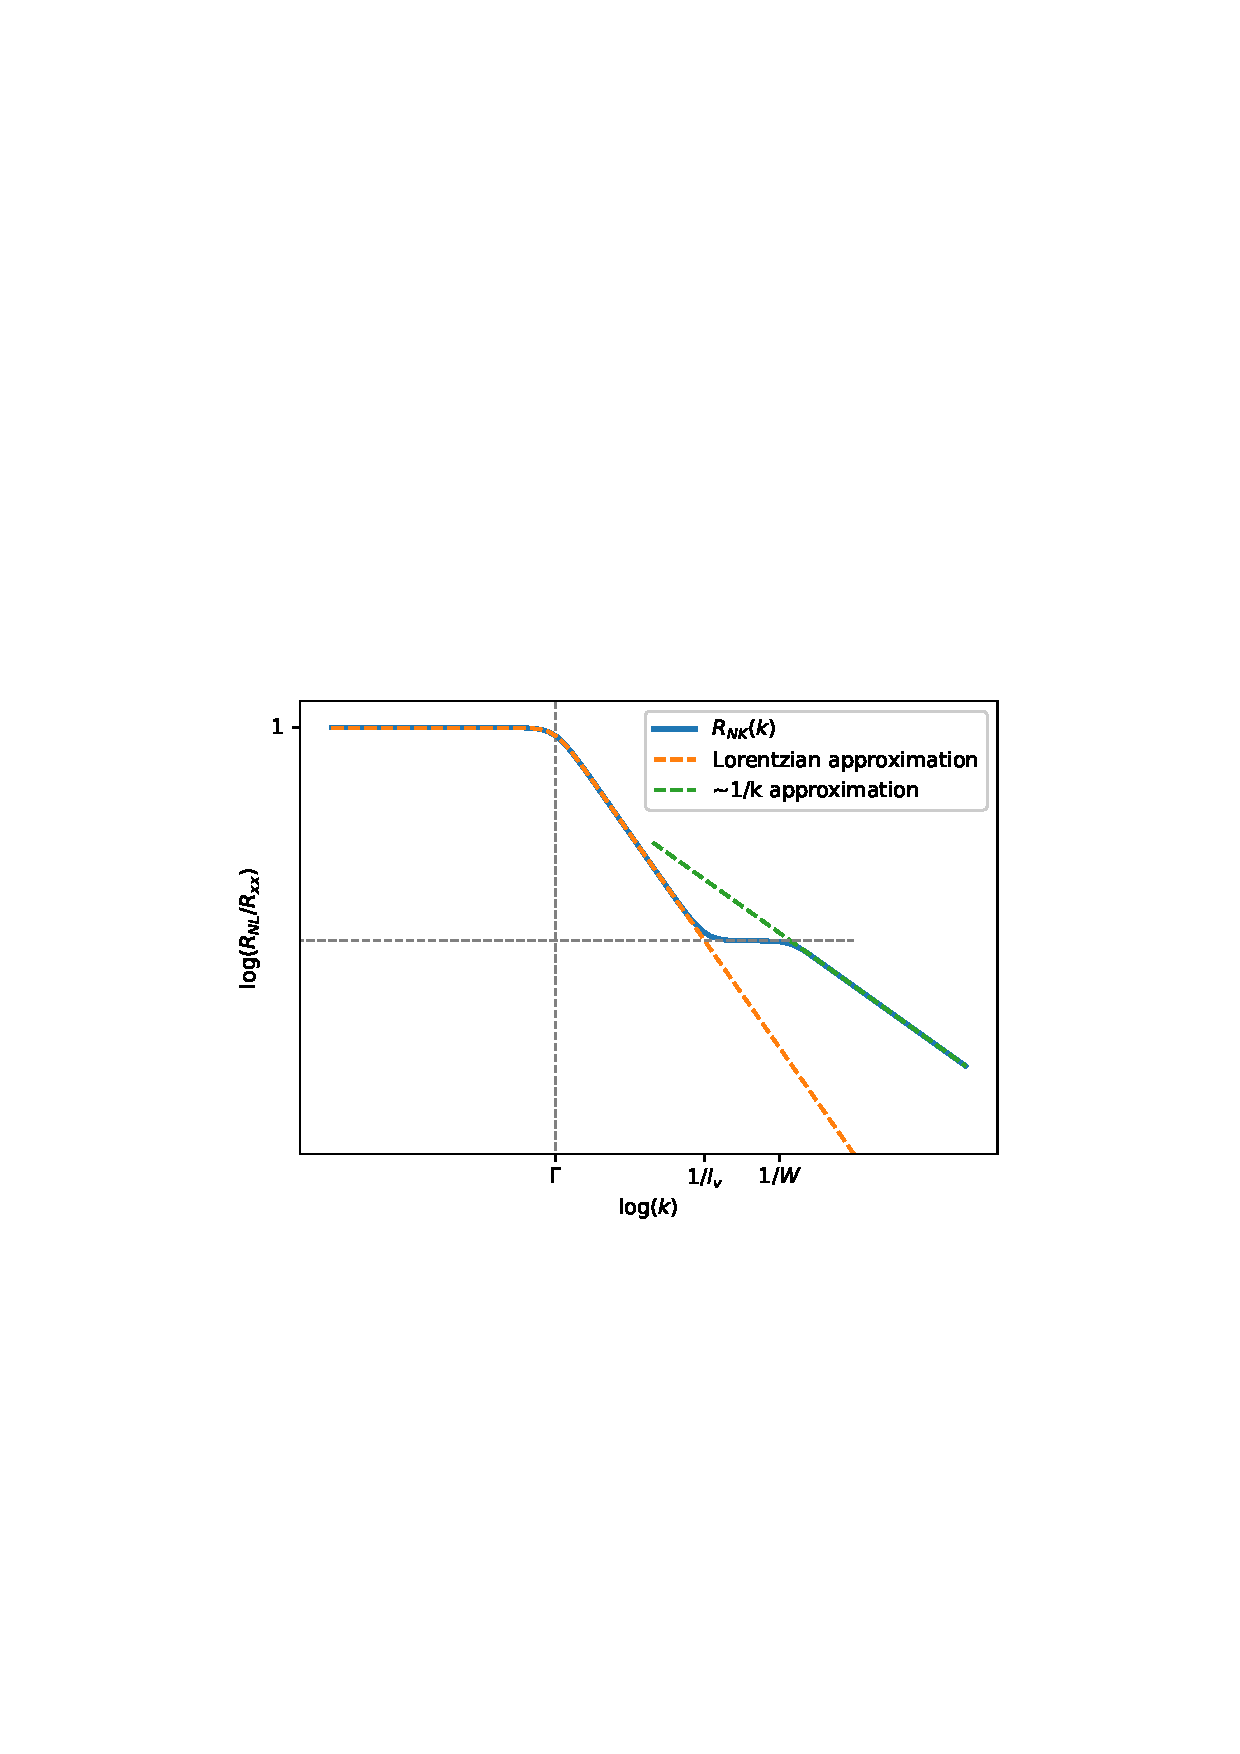
\includegraphics[width=\linewidth]{Immagini/rnl/rho3.pdf}
    \caption{The main regimes of this function}
    \label{fig:rho3}
\end{figure}\\
Notice how the equations for the second and third regime are both proportional to $\rho/(1+\tan^2(\theta_{VH}))$. This means we can write equation \ref{eq:rhotoinf} as approximately
\begin{equation}
    \lim_{\rho\to\infty} R_{NL}(k)=\frac{R_{xx}}{1+(k/\sigma)^2} + \frac \rho{1+\tan^2(\theta_{VH})}C(k)
    \label{eq:rhotoinf2}
\end{equation}
Where $C(k)$ is a function that doesn't depend on $\rho$ or $\tan(\theta_{VH})$ and it comprehends the second, third regime and eventual corrections in between the approximations\footnote{Yes, the corrections also are proportional to $\rho/(1+\tan^2(\theta_{VH}))$ SPIEGA PERCHè}.\\
Now let $G(x)$ be it's Fourier anti-transform, then we have that 

\begin{equation}
    \lim_{\rho\to\infty} R_{NL}(x)=S + \frac 1\rho G(x)
\end{equation}
This means that for $\rho\to +\infty$ the right hand side term vanishes, unless it diverges. And indeed $G(x)$ diverges for $x=0$. Therefore the limit above has pointwise convergence in $\{x\in \mathbb R\,|\,x\neq 0\}$
\begin{figure}[h!]
    \centering
    \includegraphics[width=\linewidth]{Immagini/rnl/all_approx_rho.pdf}
    \caption{The main regimes of this function}
    \label{fig:all_approx_rho}
\end{figure}\\

\section{Comparison with experimental data}
